
% This LaTeX was auto-generated from an M-file by MATLAB.
% To make changes, update the M-file and republish this document.

\documentclass{article}
\usepackage{graphicx}
\usepackage{color}

\sloppy
\definecolor{lightgray}{gray}{0.5}
\setlength{\parindent}{0pt}

\begin{document}

    
    
\section*{Simple calibration of a 1D analytic model}

\begin{par}
TO May 2013
\end{par} \vspace{1em}

\subsection*{Contents}

\begin{itemize}
\setlength{\itemsep}{-1ex}
   \item Intro
   \item Parameters used in the calibration
   \item Initial parameter values and perturbations
   \item Change of default of model parameters, add any (see model for possible parameters
   \item Number of observations and measurement locatons
   \item Initial parameter vectors, usage above determines which ones are used.
   \item Generate synthetic measurements
   \item Offset from true parameters (implemented in terms of multiplyers
   \item True parameters that will make the model equal to the measurements
   \item True model without random errors
   \item Add synthetic random errors to yM if necessary
   \item Initial parameters and model outcome
   \item Sensitivities computation (Jacobian)
   \item perturbation of model parameter values
   \item Compute Jacobian matrix (sensitivities)
   \item Optimal update of initial parameters
   \item Show results for comparison
   \item Covariance matrix and other statistics
   \item Display results
   \item Issue results for the parameters in readable format
   \item The next step
\end{itemize}


\subsection*{Intro}

\begin{par}
The model is a 1D steady state phreatic head between two ditches at distance L. We have a fixed head in the ditches. The conductivity is kL between xL\ensuremath{<}alpha*L and kR voor x\ensuremath{>}alpha*L. The bottom of the aquifer is at zB = -13. Free parameters are kL kR alpha and zB.
\end{par} \vspace{1em}
\begin{par}
We set up a calibration from scratch. Linearizing the relatin between model parameters and the outcomes at measurement locations and then updating the parameter vector such that we get a good fit between model and measurements. We use one step only. In this case we get generally a good fit. Clearly, because the relation between model parameters and heads is non-linear, we should repeat this procedure several times in real-world situation. Whether we reach a minimum or not, depends on the shape of the cost function and the method that is applied to reach such a minimum. The Marqardt-Levenber methed is the most applied non-linear search method, which is a weighted mix of steepest decend and the method shown here using the linearization and solving for the parameter vector update. The Marquardt-Levenberg methods is implemented in the Matlab function lsqnonlin (least squares non linear). This method is used in the other script called CalibNonLin in this same directory. It uses parObj to define parameters and is quite generic, so that with little effort much more complicated models may be calibrated.
\end{par} \vspace{1em}
\begin{par}
In the current file we use a simple approach, with no fancy objects, so that every step is transparent.
\end{par} \vspace{1em}
\begin{verbatim}
% TO 130619

clear variables
\end{verbatim}


\subsection*{Parameters used in the calibration}

\begin{verbatim}
usage =    [ 1    0       1    1 ];  % set to 0 to switch off and 1 to switch on
parname = {'kL','kR','alpha','zB'};  % the switches pertain to these parameters

use = usage~=0;  % Use is now a logical array telling which of the parmeters
                 % will be calibrated and which not.
\end{verbatim}


\subsection*{Initial parameter values and perturbations}

\begin{verbatim}
kL    = 1;       dkL = 0.05*kL;
kR    = 20;      dkR = 0.05*kR;
alpha = 0.25;    da  = 0.05*alpha;
zB    = -10;     dzB = 0.05*zB;
\end{verbatim}


\subsection*{Change of default of model parameters, add any (see model for possible parameters}

\begin{verbatim}
L     = 1000;
defaults = {'L',L};
\end{verbatim}


\subsection*{Number of observations and measurement locatons}

\begin{verbatim}
Np    = 50;
xM    = unique(L * rand(Np,1));  % random locations between 0 and L
\end{verbatim}


\subsection*{Initial parameter vectors, usage above determines which ones are used.}

\begin{verbatim}
p0  =[kL kR alpha zB]';  % initial paramter vector
dp0 =[dkL dkR da dzB];   % change applied to compute sensitivity (Jacobian)
\end{verbatim}


\subsection*{Generate synthetic measurements}

\begin{par}
The measurements are generated using the model in "model.m" with its parameters a bit offset from the "true" parameters and with random errors added.
\end{par} \vspace{1em}


\subsection*{Offset from true parameters (implemented in terms of multiplyers}

\begin{verbatim}
off_kL    =-0.2*kL;
off_kR    = 0.2*kR;
off_alpha = 0.2*alpha;
off_zB    = 0.0*zB;
\end{verbatim}


\subsection*{True parameters that will make the model equal to the measurements}

\begin{verbatim}
pTrue = [kL+off_kL,kR+off_kR,alpha+off_alpha,zB+off_zB]';
\end{verbatim}


\subsection*{True model without random errors}

\begin{verbatim}
yM = model('xM',xM,'kL',kL+off_kL,'kR',kR+off_kR,'alpha',alpha+off_alpha,'zB',zB+off_zB,defaults{:});
\end{verbatim}


\subsection*{Add synthetic random errors to yM if necessary}

\begin{verbatim}
try   % try to load random errors (to keep them the same all the time)
    load randErrors
    if numel(yM)~=numel(randErrors)
        error('Generating random errors');
    end
    fprintf('Random errors loaded.\n');
catch ME  % renew random errors
    fprintf('%s\nGenerating and saving random errors.',ME.message);
    randErrors = 0.05*randn(size(yM));
    save randErrors randErrors;
end

% simulated measurements
yM = yM + randErrors;
\end{verbatim}

        \color{lightgray} \begin{verbatim}Random errors loaded.
\end{verbatim} \color{black}
    

\subsection*{Initial parameters and model outcome}

\begin{par}
The initial parameters for the calibration were given above. We have at most 4 parameters in this model kL kR alpha and zB. The active ones are selected with the usage near the top of this file.
\end{par} \vspace{1em}


\subsection*{Sensitivities computation (Jacobian)}

\begin{verbatim}
% Model outcome for initial parameters
y0=  model('xM',xM,'kL',kL,'kR',kR,'alpha',alpha,'zB',zB,defaults{:});
\end{verbatim}


\subsection*{perturbation of model parameter values}

\begin{par}
Run model for all parameters in turn with a small value change
\end{par} \vspace{1em}
\begin{verbatim}
sp= [
    model('xM',xM,'kL',kL+dkL,'kR',kR,'alpha',alpha,'zB',zB,defaults{:}),... % par1
    model('xM',xM,'kL',kL,'kR',kR+dkR,'alpha',alpha,'zB',zB,defaults{:}),... % par2
    model('xM',xM,'kL',kL,'kR',kR,'alpha',alpha+da,'zB',zB,defaults{:}),...  % par3
    model('xM',xM,'kL',kL,'kR',kR,'alpha',alpha,'zB',zB+dzB,defaults{:})     % par4
    ];
\end{verbatim}


\subsection*{Compute Jacobian matrix (sensitivities)}

\begin{verbatim}
J = bsxfun(@rdivide,bsxfun(@minus,sp(:,use),y0),dp0(use));
\end{verbatim}


\subsection*{Optimal update of initial parameters}

\begin{verbatim}
Inv    = (J'*J)^(-1);
B      = Inv*J';

dp     = B *(yM-y0); % dp  = (J'*J)^(-1)*J' * (yM-y0)

y      = y0+J*dp;     % end results, initial + update through parameter change
p      = p0(use)+dp;  % end results for parameters
\end{verbatim}


\subsection*{Show results for comparison}

\begin{verbatim}
fsz = 14; % fontsize used in plot

figure; axes('nextplot','add','fontsize',fsz);
xlabel('x [m]','fontsize',fsz);
ylabel('head [m]','fontsize',fsz);
title('Calibration: Head in measurement points','fontsize',fsz);

plot(xM,yM,'bx');  % model measured data
plot(xM,y0,'ro');  % model initial parameters
plot(xM,y ,'gs');  % model optimized parameters
legend('measured','initial','optmized');
\end{verbatim}

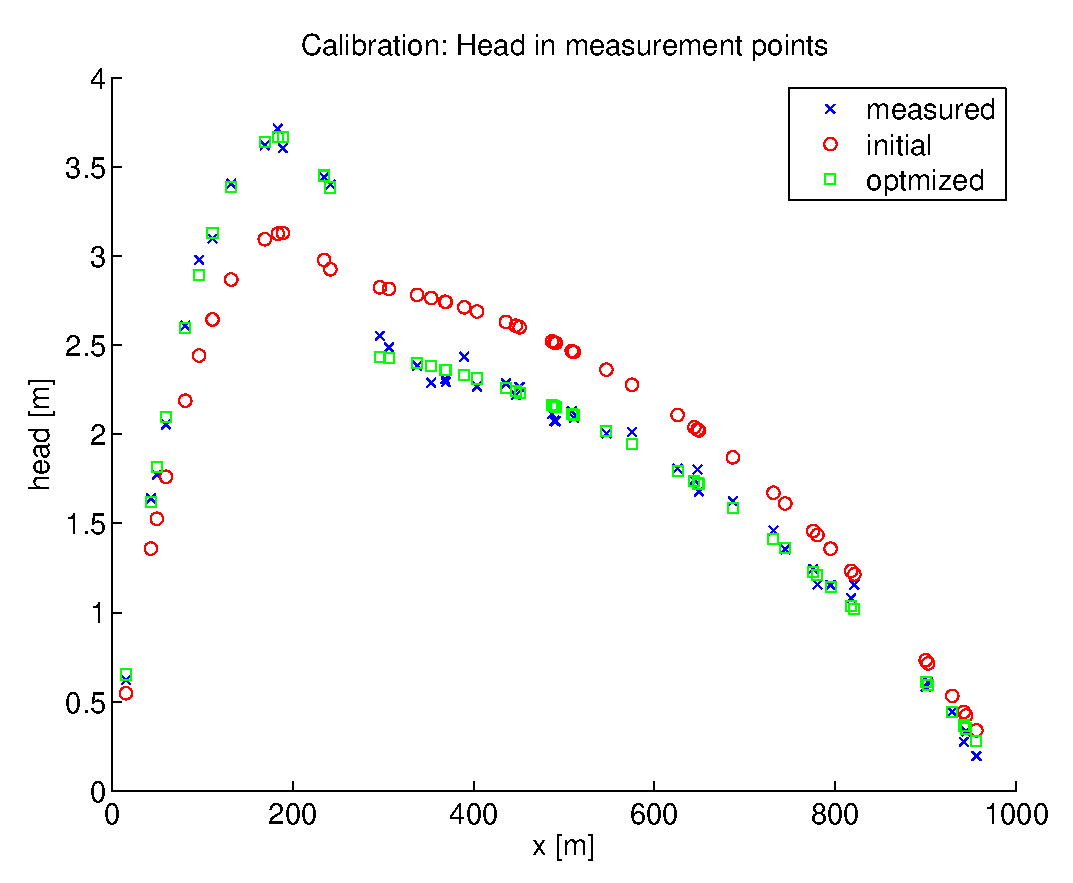
\includegraphics [width=4in]{CalibSimple_01.eps}


\subsection*{Covariance matrix and other statistics}

\begin{verbatim}
e      = (yM-y);                % heads errors, measured - computed
sigma  = std(e);                % errors in heads after calibration
Cov    = sigma^2*Inv;           % covariance matrix of the parameters
sigmaP = sqrt(diag(Cov));       % std of the parameters
uncert = 100*sigmaP./abs(p);    % uncertainty
Cor    = Cov./(sigmaP*sigmaP'); % correlation matrix of the parameters
\end{verbatim}


\subsection*{Display results}

\begin{verbatim}
display(Cov);
display(Cor);
\end{verbatim}

        \color{lightgray} \begin{verbatim}
Cov =

    0.0010    0.0001    0.0019
    0.0001    0.0000    0.0002
    0.0019    0.0002    0.0060


Cor =

    1.0000    0.7193    0.7899
    0.7193    1.0000    0.4342
    0.7899    0.4342    1.0000

\end{verbatim} \color{black}
    

\subsection*{Issue results for the parameters in readable format}

\begin{verbatim}
fprintf('results: error = %.4g m\nUncertainty = 100*sigmaP/abs(p)\n',sigma);
fprintf('%10s%10s%10s%10s%10s%10s\n','parameter','pTrue','pInit','pEnd','sigmaP','uncert%');
k=0;
for i=find(use)
    k=k+1;
    fprintf('%10.4s',parname{i});
    fprintf('%10.4g',pTrue(i));
    fprintf('%10.4g',p0(i));
    fprintf('%10.4g',p(k));
    fprintf('%10.4g',sigmaP(k));
    fprintf('%10.4g',uncert(k));
    fprintf('\n');
end
\end{verbatim}

        \color{lightgray} \begin{verbatim}results: error = 0.0541 m
Uncertainty = 100*sigmaP/abs(p)
 parameter     pTrue     pInit      pEnd    sigmaP   uncert%
        kL       0.8         1    0.5767   0.03113     5.398
      alph       0.3      0.25    0.3384  0.004753     1.404
        zB       -10       -10    -11.96   0.07736    0.6468
\end{verbatim} \color{black}
    

\subsection*{The next step}

\begin{par}
the next step is to change the initial parameters into the correct direction This is done in mfCalib, using Matlab's lsqnonlin solver.
\end{par} \vspace{1em}



\end{document}
    
